\section{PROGRAMACIÓN EXTREMA (XP)}

Citando a \parencite{solis2003XP}, la \textit{Programación Extrema} es una metodología de desarrollo de software que se basa en la simplicidad, la comunicación y el reciclado continuo de código. Además, siguiendo a \parencite{pressman2010ingenieria}, se dice que \textit{XP} es el enfoque más utilizado del desarrollo de software ágil.

Los objetivos de \textit{XP} se centran en la satisfacción del cliente, enfocandose en entregar un producto alineado con las necesidades del cliente.

\textbf{VALORES XP}

En \parencite{pressman2010ingenieria} se define un conjunto de cinco valores que establecen el fundamento para los desarrollos basados en \textit{XP}: comunicación, simplicidad, retroalimentación, valentía y respeto.

\begin{itemize}
    \item Para lograr la \textbf{Comunicación} entre los integrantes del equipo del desarrollo y agentes externos, se pone el énfasis en la colaboración estrecha entre los clientes y los desarrolladores para comunicar conceptos importantes y retroalimentación continua.
    \item La \textbf{Simplicidad} se logra restringiendo a los desarrolladores para que diseñen sólo para las necesidades inmediatas, en lugar de considerar las del futuro. Si se necesita mejorar el diseño, se realizarán las mejoras en el futuro.
    \item Para fomentar la \textbf{Retroalimentación} se definen tres fuentes esenciales: El software implementado, el cliente y otros miembros del equipo. El software brinda retroalimentación mediante \textit{priebas unitarias}.
    \item Seguir la metodología \textit{XP} requiere de \textbf{Valentía o Disciplina}. Un equipo \textit{XP} debe tener la valentía de diseñar centrándose en el hoy y reconocer que los requerimientos futuros podrían cambiar mucho y deberán modificar el diseño y código implementado.
    \item Para apegarse a cada una de las reglas \textit{XP} se requiere \textbf{Respeto} entreo los miembros del equipo e indirectamente para el software en sí mismo.
\end{itemize}

\textbf{FASES DE LA PROGRAMACIÓN EXTREMA}

La \textit{Programación Extrema} engloba un conjunto de reglas y prácticas que ocurren en el contexto de cuatro actividades estructurales representadas en la \Cref{fig:XPFases}. A continuación se describen de manera general las fases inherentes a \textit{XP}.

\begin{figure}[h!]
    \centering
    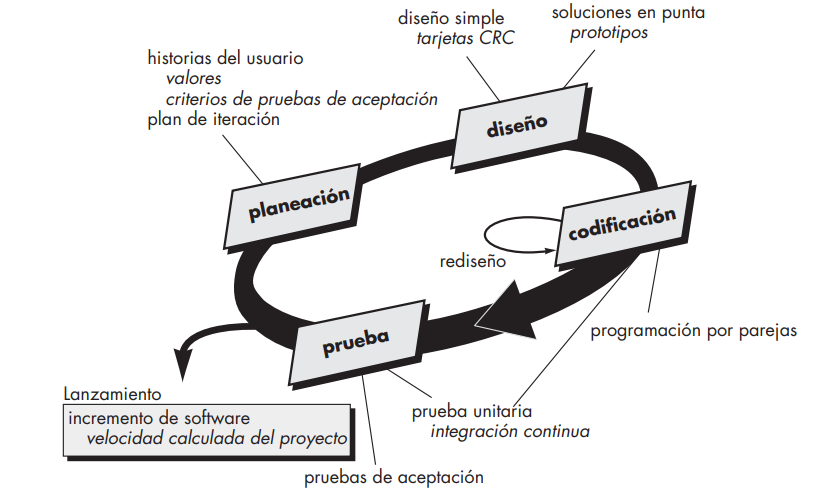
\includegraphics[width=1\linewidth]{XPFases.png}
    \caption{Fases de la Programación Extrema \parencite{pressman2010ingenieria}.}
    \label{fig:XPFases}
\end{figure}

\textbf{PLANEACIÓN}

Según \parencite{solis2003XP}, la planificación está planteada como un permanente diálogo entre la parte empresarial (lo deseable) y la técnica (lo posible).
Esta actividad comienza recabando los requerimientos para que el equipo de trabajo entiendan el contexto del negocio para el software. 

Basándose en \parencite{pressman2010ingenieria}, la planeación permite escuchar y recabar \textit{historias de usuario} que describen la salida necesaria, características y funcionalidad del software que se va a elaborar. Cada historia es descrita por el cliente. Es importante mencionar que en cualquier momento es posible escribir nuevas historias.

Además, el cliente (o persona del negocio) debe determinar lo siguiente:

\begin{itemize}
    \item \textbf{Ámbito:} ¿Qué es lo que el software debe de resolver para que genere valor?
    \item \textbf{Prioridad: } ¿Qué debe ser hecho en primer lugar?
    \item \textbf{Composición de Versiones: } ¿Cuánto es necesario hacer para saber si el negocio va mejor con el software que sin él?
    \item \textbf{Estimaciones: } ¿Cuánto tiempo lleva iplementar una característica?
    \item \textbf{Procesos: } ¿Cómo se organiza el trabajo y el equipo?
\end{itemize}

A medida que avanza el trabajo, el cliente puede agregar historias, cambiar el valor de una ya existente, descomponerlas o eliminarlas \parencite{pressman2010ingenieria}.

\textbf{DISEÑO}

El diseño en \textit{XP} se basa en el principio de \textit{`Mantenlo Sencillo`} que se basa en las siguientes reglas \parencite{solis2003XP}:

\begin{enumerate}
    \item Funciona con todas las pruebas.
    \item No tiene lógica duplicada.
    \item Manifiesta cada intención importante para los programadores.
    \item Tiene el menor número de clases y métodos.
\end{enumerate}

Según \parencite{pressman2010ingenieria}, un concepto central en \textit{XP} es que el diseño ocurre tanto antes como después de que comienza la codificación. Rediseñar significa que el diseño se hace de manera continua conforme se construye el sistema.

\textbf{CODIFICACIÓN}

La codificación en \textit{XP} se centra en historias validadas por pruebas unitarias, siendo fiel al diseño fundamental sin agregar nada extraño. El planteamiento de codificación más relevante es intentar implementar funcionalidades de la manera más simple posible. Después de implementar nuevas características, es necesario preguntarse cómo hacer el programa más simple sin perder funcionalidad \parencite{solis2003XP}.

\newpage

\textbf{PRUEBAS}

Según \parencite{pressman2010ingenieria}, las pruebas que se crean deben implementarse con el uso de una estructura que permita la automatización. 
No debe existir ninguna característica en el programa que no haya sido probada, los programadores escriben pruebas para verificar el correcto funcionamiento del programa, los clientes realizan pruebas funcionales. El resultado deriva a un programa más seguro que conforme pasa el tiempo es capaz de aceptar nuevos cambios.

La metodología \textit{XP} parece arriesgada y voráz porque apuesta por velocidad, simpleza y cambios continuos, sin emabargo, en entornos reales ese riesgo se disuelve con prácticas técnicas estrictas que protegen el desarrollo.

